\documentclass[conference]{IEEEtran}
\IEEEoverridecommandlockouts

\usepackage[utf8]{inputenc}
\usepackage[turkish,shorthands=off]{babel}
\usepackage{cite}
\usepackage{amsmath,amssymb,amsfonts}
\usepackage{algorithmic}
\usepackage{algorithm}
\usepackage{graphicx}
\usepackage{textcomp}
\usepackage{xcolor}
\usepackage{booktabs}
\usepackage{url}
\usepackage{float}
\usepackage{multirow}

\begin{document}

\title{Depo Yeri Se\c{c}imi Problemi i\c{c}in Hibrit Yakla\c{s}{\i}m:\\
K-Means K\"{u}meleme ve A\c{c}g\"{o}zl\"{u} Algoritma Entegrasyonu}

\author{
\IEEEauthorblockN{\"{O}mer Faruk DAMAR}
\IEEEauthorblockA{
  Yaz{\i}l{\i}m M\"{u}hendisli\u{g}i B\"{o}l\"{u}m\"{u}\\
  Manisa Celal Bayar \"{U}niversitesi\\
  Hasan Ferdi Turgutlu Teknoloji Fak\"{u}ltesi\\
  Manisa, T\"{u}rkiye}
\and
\IEEEauthorblockN{Mehmet Ali AVCI}
\IEEEauthorblockA{
  Yaz{\i}l{\i}m M\"{u}hendisli\u{g}i B\"{o}l\"{u}m\"{u}\\
  Manisa Celal Bayar \"{U}niversitesi\\
  Hasan Ferdi Turgutlu Teknoloji Fak\"{u}ltesi\\
  Manisa, T\"{u}rkiye}
}

\maketitle

\begin{abstract}
Bu \c{c}al{\i}\c{s}mada, tedarik zinciri optimizasyonunun temel NP-zor
problemlerinden biri olan Depo Yeri Se\c{c}imi Problemi (Warehouse Location
Problem -- WLP) ele al{\i}nmaktad{\i}r.
Problemin \c{c}\"{o}z\"{u}m\"{u} i\c{c}in K-Means k\"{u}meleme algoritmas{\i}
ile A\c{c}g\"{o}zl\"{u} (Greedy) atama yakla\c{s}{\i}m{\i}n{\i} birle\c{s}tiren
ve takas tabanl{\i} yerel iyile\c{s}tirme ad{\i}m{\i} i\c{c}eren hibrit bir
y\"{o}ntem \"{o}nerilmektedir.
\"{O}nerilen y\"{o}ntemde m\"{u}\c{s}teri konumlar{\i} \"{o}nce K-Means ile
anlaml{\i} k\"{u}melere ayr{\i}lmakta, ard{\i}ndan her k\"{u}me merkezine en
yak{\i}n aday depo A\c{c}g\"{o}zl\"{u} y\"{o}ntemle se\c{c}ilmektedir.
Y\"{o}ntemin performans{\i}; saf A\c{c}g\"{o}zl\"{u} algoritma, Rastgele
Arama (Random Search) ve Tam Say{\i}l{\i} Programlama (Integer Programming~--
IP) ile \"{u}\c{c} farkl{\i} \"{o}l\c{c}ek d\"{u}zeyinde (50, 100 ve 200
m\"{u}\c{s}teri) kar\c{s}{\i}la\c{s}t{\i}rmal{\i} olarak
de\u{g}erlendirilmektedir.
$K \in \{2,\ldots,8\}$ depo say{\i}s{\i} \"{u}zerinde ger\c{c}ekle\c{s}tirilen
deneyler; hibrit y\"{o}ntemin saf A\c{c}g\"{o}zl\"{u} algoritmay{\i}
b\"{u}y\"{u}k \"{o}l\c{c}ekte geride b{\i}rakt{\i}\u{g}{\i}n{\i},
Rastgele Arama'ya k{\i}yasla b\"{u}y\"{u}k veri setlerinde daha d\"{u}\c{s}\"{u}k
maliyet elde etti\u{g}ini ve IP ile k{\i}yaslanabilir kalite sunarken
hesaplama s\"{u}resini \c{c}ok daha d\"{u}\c{s}\"{u}k tuttu\u{g}unu
ortaya koymaktad{\i}r.
\end{abstract}

\begin{IEEEkeywords}
Depo Yeri Se\c{c}imi Problemi, K-Means K\"{u}meleme, A\c{c}g\"{o}zl\"{u}
Algoritma, Hibrit Optimizasyon, Tam Say{\i}l{\i} Programlama, NP-Zor Problem,
Yerel Arama, Tedarik Zinciri
\end{IEEEkeywords}

\section{Giri\c{s}}

Lojistik ve tedarik zinciri y\"{o}netiminde al{\i}nan kararlar{\i}n kalitesi,
i\c{s}letme maliyetleri \"{u}zerinde do\u{g}rudan belirleyici bir etkiye
sahiptir.
Bu kararlar{\i}n en kritiklerinden biri, m\"{u}\c{s}teri talep noktalar{\i}n{\i}
en d\"{u}\c{s}\"{u}k toplam maliyetle kar\c{s}{\i}layacak depolar{\i}n
konumland{\i}r{\i}lmas{\i}d{\i}r.
Depo Yeri Se\c{c}imi Problemi (WLP), sabit a\c{c}{\i}l{\i}\c{s} ve ta\c{s}{\i}ma
maliyetleri toplam{\i}n{\i} minimize eden depo k\"{u}mesini belirleme
amac{\i}n{\i} ta\c{s}{\i}yan, NP-zor s{\i}n{\i}f{\i}nda bir kombinatoryal
optimizasyon problemidir~\cite{cornuejols1977}.
Bu s{\i}n{\i}fland{\i}rma, b\"{u}y\"{u}k \"{o}l\c{c}ekli \"{o}rnekler
i\c{c}in tam (kesin) \c{c}\"{o}z\"{u}m y\"{o}ntemlerini hesaplama
s\"{u}resi a\c{c}{\i}s{\i}ndan uygulanamaz k{\i}lmakta~\cite{garey1979};
sezgisel ve meta-sezgisel yakla\c{s}{\i}mlar{\i} zorunlu hale getirmektedir.

Bu \c{c}al{\i}\c{s}man{\i}n temel katk{\i}s{\i}, literat\"{u}rde
ba\u{g}{\i}ms{\i}z olarak incelenen K-Means k\"{u}meleme~\cite{lloyd1982}
ve Greedy atama yakla\c{s}{\i}mlar{\i}n{\i} WLP'\''ye \"{o}zg\"{u} bir
hibrit \c{c}er\c{c}evede birle\c{s}tirmektir.
\"{O}nerilen y\"{o}ntem \"{u}\c{c} ana bile\c{s}enden olu\c{s}maktad{\i}r:
\textit{(i)}~K-Means ile m\"{u}\c{s}teri noktalar{\i}n{\i} do\u{g}al
k\"{u}melere ay{\i}rma,
\textit{(ii)}~her k\"{u}me merkezi i\c{c}in Greedy kriteriyle en uygun
aday depoyu belirleme ve
\textit{(iii)}~kapasite ihlallerini gidermek i\c{c}in takas tabanl{\i}
yerel arama uygulamas{\i}.

Kar\c{s}{\i}la\c{s}t{\i}rmal{\i} deneyler; hibrit y\"{o}ntemin saf
A\c{c}g\"{o}zl\"{u} algoritmaya k{\i}yasla belirgin bi\c{c}imde \"{u}st\"{u}n
sonu\c{c}lar \"{u}retti\u{g}ini, Rastgele Arama ile rekabet etti\u{g}ini
ve tam \c{c}\"{o}z\"{u}m y\"{o}ntemine (IP) k{\i}yasla \c{c}ok daha az
hesaplama kayna\u{g}{\i} gerektirdi\u{g}ini g\"{o}stermektedir.

\c{C}al{\i}\c{s}man{\i}n geri kalan b\"{o}l\"{u}mleri \c{s}u \c{s}ekilde
d\"{u}zenlenmi\c{s}tir:
B\"{o}l\"{u}m~\ref{sec:lit} literat\"{u}r taramas{\i}n{\i},
B\"{o}l\"{u}m~\ref{sec:method} \"{o}nerilen y\"{o}ntemi,
B\"{o}l\"{u}m~\ref{sec:exp} deneysel sonu\c{c}lar{\i} ve
B\"{o}l\"{u}m~\ref{sec:conc} sonu\c{c} ve gelecek \c{c}al{\i}\c{s}malar{\i}
sunmaktad{\i}r.

\section{Literat\"{u}r Taramas{\i}}
\label{sec:lit}

WLP ve t\"{u}revleri \"{u}zerine kapsaml{\i} \c{c}al{\i}\c{s}malar
mevcuttur.
Cornuejols ve ark.~\cite{cornuejols1977} sabit maliyetli tesis
konumland{\i}rma problemleri i\c{c}in polinom zamanl{\i} yakla\c{s}{\i}m
algoritmalar{\i}n{\i} incelemi\c{s} ve \c{c}e\c{s}itli alt problemlerin
NP-zorlu\u{g}unu kan{\i}tlam{\i}\c{s}t{\i}r.
Kuehn ve Hamburger~\cite{kuehn1963}, depo konumland{\i}rmas{\i} i\c{c}in
erken d\"{o}nemin en etkili Greedy sezgiseli olan PLANT modelini
geli\c{s}tirmi\c{s}; bu \c{c}al{\i}\c{s}ma g\"{u}n\"{u}m\"{u}z
sezgisel ara\c{s}t{\i}rmalar{\i}na temel te\c{s}kil etmektedir.

K\"{u}meleme y\"{o}ntemleri ile tesis konumland{\i}rma aras{\i}ndaki ili\c{s}ki
Kaufman ve Rousseeuw~\cite{kaufman1990} taraf{\i}ndan kapsaml{\i} bi\c{c}imde
ele al{\i}nm{\i}\c{s}t{\i}r.
Resende ve Werneck~\cite{resende2004} ise p-medyan problemine y\"{o}nelik
hibrit bir sezgisel geli\c{s}tirerek k\"{u}meleme ile yerel araman{\i}n
sinerjisini ortaya koymu\c{s}tur.
Daskin~\cite{daskin2011}, a\u{g} ve ayr{\i}k konum problemleri \"{u}zerine
kapsaml{\i} bir \c{c}er\c{c}eve sunarak WLP'\''nin farkl{\i} varyantlar{\i}n{\i}
sistematik olarak s{\i}n{\i}fland{\i}rm{\i}\c{s}t{\i}r.

Tam say{\i}l{\i} programlama y\"{o}ntemleri a\c{c}{\i}s{\i}ndan
Benders~\cite{benders1962} ayr{\i}\c{s}t{\i}rma y\"{o}ntemi WLP'\''ye
uyarlanm{\i}\c{s} ve b\"{u}y\"{u}k \"{o}rneklerde etkin sonu\c{c}lar
vermi\c{s}tir.
Meta-sezgisel y\"{o}ntemler a\c{c}{\i}s{\i}ndan Gendreau ve
ark.~\cite{gendreau1996} tabu araman{\i}n WLP benzeri problemlere
uygulanmas{\i}n{\i} incelemi\c{s}; elde edilen sonu\c{c}lar yerel
minimumlardan ka\c{c}{\i}n{\i}mda tabu araman{\i}n belirgin katk{\i}
sa\u{g}lad{\i}\u{g}{\i}n{\i} g\"{o}stermi\c{s}tir.
Son y{\i}llarda derin pekiştirmeli \"{o}\u{g}renme tabanl{\i} yakla\c{s}{\i}mlar
da tesis konumland{\i}rma problemlerinde umut verici sonu\c{c}lar
vermektedir~\cite{nazari2018}; ancak bu y\"{o}ntemler yo\u{g}un e\u{g}itim
s\"{u}resi gerektirmekte ve k\"{u}\c{c}\"{u}k--orta \"{o}l\c{c}ekli
problemlerde klasik sezgisellerle rekabet edememektedir.

Bu \c{c}al{\i}\c{s}ma, s\"{o}z konusu birikimden hareketle K-Means \"{o}nc\"{u}
a\c{s}amas{\i}n{\i}, Greedy atamay{\i} ve takas tabanl{\i} yerel arama
ad{\i}m{\i}n{\i} birle\c{s}tiren; IP ile do\u{g}rudan kar\c{s}{\i}la\c{s}t{\i}rmal{\i}
eksiksiz bir deneysel analiz sunan \"{o}zg\"{u}n bir hibrit mimari
\"{o}nermektedir.

\section{Y\"{o}ntem}
\label{sec:method}

\subsection{Problem Tan{\i}m{\i}}

WLP a\c{s}a\u{g}{\i}daki \c{s}ekilde bi\c{c}imsel olarak tan{\i}mlanabilir.
$I = \{1,\ldots,m\}$ m\"{u}\c{s}teri k\"{u}mesi ve
$J = \{1,\ldots,n\}$ aday depo k\"{u}mesi olmak \"{u}zere:
$d_i$ m\"{u}\c{s}teri $i$'\''nin talebini,
$f_j$ depo $j$'\''nin sabit a\c{c}{\i}l{\i}\c{s} maliyetini,
$c_{ij}$ m\"{u}\c{s}teri $i$'\''yi depo $j$'\''ye atama (ta\c{s}{\i}ma)
maliyetini,
$s_j$ depo $j$'\''nin kapasitesini g\"{o}stermektedir.
Karar de\u{g}i\c{s}kenleri:
$y_j \in \{0,1\}$ depo $j$'\''nin a\c{c}{\i}l{\i}p a\c{c}{\i}lmad{\i}\u{g}{\i}n{\i},
$x_{ij} \in \{0,1\}$ m\"{u}\c{s}teri $i$'\''nin depo $j$'\''ye
atanmas{\i}n{\i} g\"{o}stermektedir.

Ama\c{c} fonksiyonu:
\begin{equation}
  \min \sum_{j \in J} f_j y_j +
       \sum_{i \in I}\sum_{j \in J} d_i\, c_{ij}\, x_{ij}
  \label{eq:obj}
\end{equation}
K{\i}s{\i}tlar:
\begin{align}
  &\sum_{j \in J} x_{ij} = 1, \quad \forall i \in I
  \label{eq:assign}\\
  &x_{ij} \leq y_j, \quad \forall i \in I,\; j \in J
  \label{eq:open}\\
  &\sum_{i \in I} d_i\, x_{ij} \leq s_j\, y_j, \quad \forall j \in J
  \label{eq:cap}\\
  &\sum_{j \in J} y_j = K
  \label{eq:k}
\end{align}

Denklem~\eqref{eq:assign} her m\"{u}\c{s}terinin tam olarak bir depoya
atanmas{\i}n{\i},~\eqref{eq:open} ataman{\i}n yaln{\i}zca a\c{c}{\i}k
depoya yap{\i}labilmesini,~\eqref{eq:cap} kapasite k{\i}s{\i}tlar{\i}n{\i}
ve~\eqref{eq:k} tam olarak $K$ deponun a\c{c}{\i}lmas{\i}n{\i}
g\"{u}vence alt{\i}na al{\i}r.

\subsection{Hibrit K-Means + Greedy Algoritmas{\i}}

\"{O}nerilen yakla\c{s}{\i}m \"{u}\c{c} a\c{s}amadan olu\c{s}maktad{\i}r.

\textbf{A\c{s}ama~1 -- K-Means K\"{u}meleme:}
M\"{u}\c{s}teri koordinat vekt\"{o}rleri
$\mathbf{p}_i = (x_i,\, y_i)$ K-Means algoritmas{\i}na girdi olarak
verilir~\cite{lloyd1982} ve $K$ adet k\"{u}me elde edilir.
Her k\"{u}menin a\u{g}{\i}rl{\i}k merkezi
$\bar{\mathbf{p}}_k = \frac{1}{|C_k|}\sum_{i \in C_k}\mathbf{p}_i$
hesaplan{\i}r.
K\"{u}resel minimuma yak{\i}nsama olas{\i}l{\i}\u{g}{\i}n{\i} art{\i}rmak
i\c{c}in $n\_init{=}15$ farkl{\i} ba\c{s}lang{\i}\c{c} ile \c{c}al{\i}\c{s}t{\i}r{\i}l{\i}r.

\textbf{A\c{s}ama~2 -- Greedy Depo Se\c{c}imi:}
Her k\"{u}me merkezi $\bar{\mathbf{p}}_k$ i\c{c}in hen\"{u}z se\c{c}ilmemi\c{s}
aday depolar aras{\i}ndan \"{O}klid uzakl{\i}\u{g}{\i} en k\"{u}\c{c}\"{u}k
olan depo se\c{c}ilir:
\begin{equation}
  j^* = \underset{j \in J \setminus S}{\arg\min}\;
        \|\bar{\mathbf{p}}_k - \mathbf{w}_j\|_2
  \label{eq:greedy}
\end{equation}
burada $S$ \"{o}nceki ad{\i}mlarda se\c{c}ilmi\c{s} depolar{\i}n k\"{u}mesi,
$\mathbf{w}_j$ depo $j$'\''nin koordinat vekt\"{o}r\"{u}d\"{u}r.

\textbf{A\c{s}ama~3 -- Yerel \"{I}yile\c{s}tirme (Swap):}
\"{I}lk se\c{c}im sonucunda kapasite cezas{\i} olu\c{s}uyorsa, tek takas
(swap) operasyonlar{\i}yla iyile\c{s}tirme ger\c{c}ekle\c{s}tirilir:
se\c{c}imi iptal edilecek depo ile eklenmesi \"{o}nerilen depo belirlenir,
maliyet azal{\i}yorsa takas kal{\i}c{\i} hale getirilir ve iyile\c{s}tirme
kalmayana dek s\"{u}re\c{c} tekrarlan{\i}r.

Algoritman{\i}n s\"{o}zde kodu Algoritma~\ref{alg:hybrid}'\''de
verilmektedir.

\begin{algorithm}[H]
\caption{Hibrit K-Means + Greedy WLP}
\label{alg:hybrid}
\begin{algorithmic}[1]
\REQUIRE M\"{u}\c{s}teri koordinatlar{\i} $C$, aday depolar $W$, depo say{\i}s{\i} $K$
\ENSURE Se\c{c}ilen depo k\"{u}mesi $S$, toplam maliyet
\STATE $S \leftarrow \emptyset$
\STATE $\{C_1,\ldots,C_K\} \leftarrow$ \textsc{KMeans}$(C,\,K,\,n\_init{=}15)$
\FOR{$k = 1$ \textbf{to} $K$}
  \STATE $\bar{\mathbf{p}}_k \leftarrow$ \textsc{Centroid}$(C_k)$
  \STATE $j^* \leftarrow \arg\min_{j \in W \setminus S}
         \|\bar{\mathbf{p}}_k - \mathbf{w}_j\|_2$
  \STATE $S \leftarrow S \cup \{j^*\}$
\ENDFOR
\WHILE{iyile\c{s}tirme m\"{u}mk\"{u}n}
  \STATE $(out,\,in) \leftarrow$ \textsc{BestSwap}$(S,\,W \setminus S)$
  \IF{\textsc{Cost}$(S \setminus \{out\} \cup \{in\})
      < $ \textsc{Cost}$(S)$}
    \STATE $S \leftarrow S \setminus \{out\} \cup \{in\}$
  \ELSE
    \STATE \textbf{break}
  \ENDIF
\ENDWHILE
\RETURN $S$, \textsc{Cost}$(S)$
\end{algorithmic}
\end{algorithm}

\subsection{Kar\c{s}{\i}la\c{s}t{\i}rma Y\"{o}ntemleri}

\textbf{Greedy-Only (Saf A\c{c}g\"{o}zl\"{u}):}
T\"{u}m aday depolar $(f_j/s_j)$ oran{\i}na g\"{o}re artan s{\i}rada
s{\i}ralan{\i}r; en d\"{u}\c{s}\"{u}k orana sahip $K$ depo se\c{c}ilir.
Tek ge\c{c}i\c{s}li ve deterministik bir y\"{o}ntemdir.
Zaman karma\c{s}{\i}kl{\i}\u{g}{\i}: $O(n_w \log n_w)$.

\textbf{Rastgele Arama (Random Search):}
Her iterasyonda rastgele $K$ aday depo se\c{c}ilir;
1000 iterasyon boyunca en d\"{u}\c{s}\"{u}k maliyetli \c{c}\"{o}z\"{u}m
elde tutulur.
Arama uzay{\i}n{\i} stokastik bi\c{c}imde \"{o}rnekler.
Zaman karma\c{s}{\i}kl{\i}\u{g}{\i}: $O(n_{iter} \cdot n_c \cdot K)$.

\textbf{Tam Say{\i}l{\i} Programlama (IP):}
Denklem~\eqref{eq:obj}--\eqref{eq:k} ile tan{\i}mlanan MIP modeli
PuLP k\"{u}t\"{u}phanesi arac{\i}l{\i}\u{g}{\i}yla CBC \c{c}\"{o}z\"{u}c\"{u}s\"{u}
ile \c{c}\"{o}z\"{u}lm\"{u}\c{s}t\"{u}r.
60 saniyelik zaman s{\i}n{\i}r{\i} uygulanm{\i}\c{s};
b\"{u}y\"{u}k veri setinde $K \leq 5$ i\c{c}in \c{c}al{\i}\c{s}t{\i}r{\i}lm{\i}\c{s}t{\i}r.

\section{Deneysel Sonu\c{c}lar}
\label{sec:exp}

\subsection{Deney Kurulumu}

Deneyler \"{u}\c{c} farkl{\i} \"{o}l\c{c}ek d\"{u}zeyinde
ger\c{c}ekle\c{s}tirilmi\c{s}tir:
\textit{K\"{u}\c{c}\"{u}k}~(50~m\"{u}\c{s}teri, 10~aday depo),
\textit{Orta}~(100~m\"{u}\c{s}teri, 20~aday depo) ve
\textit{B\"{u}y\"{u}k}~(200~m\"{u}\c{s}teri, 30~aday depo).
Her veri seti i\c{c}in m\"{u}\c{s}teri konumlar{\i}, ger\c{c}ek hayat
lojistik da\u{g}{\i}l{\i}mlar{\i}n{\i} yans{\i}tmak amac{\i}yla
5~adet do\u{g}al k\"{u}me merkezi etraf{\i}nda Gaussian da\u{g}{\i}l{\i}m
($\sigma{=}10$) kullan{\i}larak $[0,100]{\times}[0,100]$ d\"{u}zleminde
\"{u}retilmi\c{s}tir.
Depo konumlar{\i} d\"{u}zg\"{u}n da\u{g}{\i}l{\i}mla belirlenmi\c{s}tir.
M\"{u}\c{s}teri talepleri $U[5,20]$, depo kapasiteleri toplam talebin
$\approx$3 kat{\i}n{\i} kar\c{s}{\i}layacak bi\c{c}imde ve sabit a\c{c}{\i}l{\i}\c{s}
maliyetleri $U[500,2000]$ aral{\i}\u{g}{\i}nda atanm{\i}\c{s}t{\i}r.
Deney say{\i}s{\i} $K \in \{2,3,4,5,6,7,8\}$ olarak belirlenmi\c{s}tir.
T\"{u}m deneyler Python~3.11 ortam{\i}nda, scikit-learn k\"{u}t\"{u}phanesi
K-Means i\c{c}in ve PuLP/CBC IP i\c{c}in kullan{\i}larak
ger\c{c}ekle\c{s}tirilmi\c{s}tir.

Performans metrikleri olarak \textit{toplam maliyet},
\textit{\c{c}al{\i}\c{s}ma s\"{u}resi (ms)} ve
\textit{optimality gap (\%)} kullan{\i}lm{\i}\c{s}t{\i}r.
Gap de\u{g}eri ayn{\i} $K$ i\c{c}in en iyi bulunan \c{c}\"{o}z\"{u}m
referans al{\i}narak hesaplanm{\i}\c{s}t{\i}r:
\begin{equation}
  \text{Gap}(\%) =
    \frac{C_{alg} - C_{ref}}{C_{ref}} \times 100
  \label{eq:gap}
\end{equation}

\subsection{Sonu\c{c} Tablolar{\i}}

Tablo~\ref{tab:kucuk}--\ref{tab:buyuk} \"{u}\c{c} veri seti i\c{c}in
elde edilen toplam maliyetleri, \c{c}al{\i}\c{s}ma s\"{u}relerini ve
optimality gap de\u{g}erlerini sunmaktad{\i}r.

\begin{table}[htbp]
\centering
\caption{K\"{u}\c{c}\"{u}k Veri Seti (50 m\"{u}\c{s}., 10 depo) --
Algoritma Performans Kar\c{s}{\i}la\c{s}t{\i}rmas{\i}}
\label{tab:kucuk}
\begin{tabular}{|c|r|r|r|r|}
\hline
\textbf{K} & \textbf{Greedy} & \textbf{Hibrit} & \textbf{Random} & \textbf{IP} \\
\hline
2 & 24,788,057 & 21,130,615 & 21,130,615 & 186,819 \\
\hline
3 &  4,685,072 &  4,362,758 &  4,362,758 &  20,198 \\
\hline
4 &  2,062,532 &  2,062,135 &  1,791,330 &  19,067 \\
\hline
5 &  2,063,625 &    291,847 &    291,847 &  19,569 \\
\hline
6 &  2,064,274 &    292,795 &    292,795 &  20,517 \\
\hline
7 &    832,119 &    293,835 &    293,835 &  21,610 \\
\hline
8 &  6,194,463 &    294,928 &    294,928 &  22,837 \\
\hline
\end{tabular}
\end{table}

\begin{table}[htbp]
\centering
\caption{Orta Veri Seti (100 m\"{u}\c{s}., 20 depo) --
Algoritma Performans Kar\c{s}{\i}la\c{s}t{\i}rmas{\i}}
\label{tab:orta}
\begin{tabular}{|c|r|r|r|r|r|r|}
\hline
\textbf{K} & \textbf{Greedy} & \textbf{Hibrit} & \textbf{Random}
           & \textbf{IP} & \textbf{H(ms)} & \textbf{IP(ms)} \\
\hline
2 & 71,864,257 & 70,713,437 & 70,713,437 &  33,769 &   9 &   196 \\
\hline
3 & 53,439,700 & 52,274,164 & 52,274,164 &  34,419 &  17 &   256 \\
\hline
4 & 45,425,534 & 34,108,542 & 35,908,172 &  40,520 &  15 &   211 \\
\hline
5 & 44,326,173 & 19,888,653 & 22,582,607 &  36,608 &  16 &   195 \\
\hline
6 & 27,195,128 & 12,933,256 & 14,027,555 &  22,342 &  21 & 43392 \\
\hline
7 & 23,086,065 &  7,032,091 & 10,215,475 &  20,734 &  25 &  1020 \\
\hline
8 & 20,386,884 &  4,310,222 &  6,719,890 &  21,242 &  34 &   580 \\
\hline
\end{tabular}
\end{table}

\begin{table}[htbp]
\centering
\caption{B\"{u}y\"{u}k Veri Seti (200 m\"{u}\c{s}., 30 depo) --
Algoritma Performans Kar\c{s}{\i}la\c{s}t{\i}rmas{\i}}
\label{tab:buyuk}
\begin{tabular}{|c|r|r|r|r|r|}
\hline
\textbf{K} & \textbf{Greedy} & \textbf{Hibrit} & \textbf{Random}
           & \textbf{IP ($K{\le}5$)} & \textbf{H(ms)} \\
\hline
2 & 184,427,030 & 179,773,719 & 179,773,719 & 103,910 &  13 \\
\hline
3 & 163,780,639 & 152,871,472 & 155,288,310 &  88,708 &  26 \\
\hline
4 & 143,761,581 & 125,990,478 & 130,132,527 &  94,149 &  42 \\
\hline
5 & 121,850,601 & 106,142,802 & 111,645,391 &  91,801 &  47 \\
\hline
6 & 120,961,540 &  87,123,566 &  89,646,434 & --- &  34 \\
\hline
7 & 106,037,267 &  68,533,154 &  73,924,590 & --- &  38 \\
\hline
8 & 106,038,007 &  46,476,546 &  62,191,540 & --- &  54 \\
\hline
\end{tabular}
\end{table}

\subsection{Grafik Analizler}

\c{S}ekil~\ref{fig:cost} algoritmalarin maliyet e\u{g}rilerini,
\c{S}ekil~\ref{fig:time} \c{c}al{\i}\c{s}ma s\"{u}relerini,
\c{S}ekil~\ref{fig:heatmap} gap {\i}s{\i} haritas{\i}n{\i},
\c{S}ekil~\ref{fig:map} depo se\c{c}im haritalari ve
\c{S}ekil~\ref{fig:scale} \"{o}l\c{c}eklenebilirlik analizini
g\"{o}stermektedir.

\begin{figure}[htbp]
  \centering
  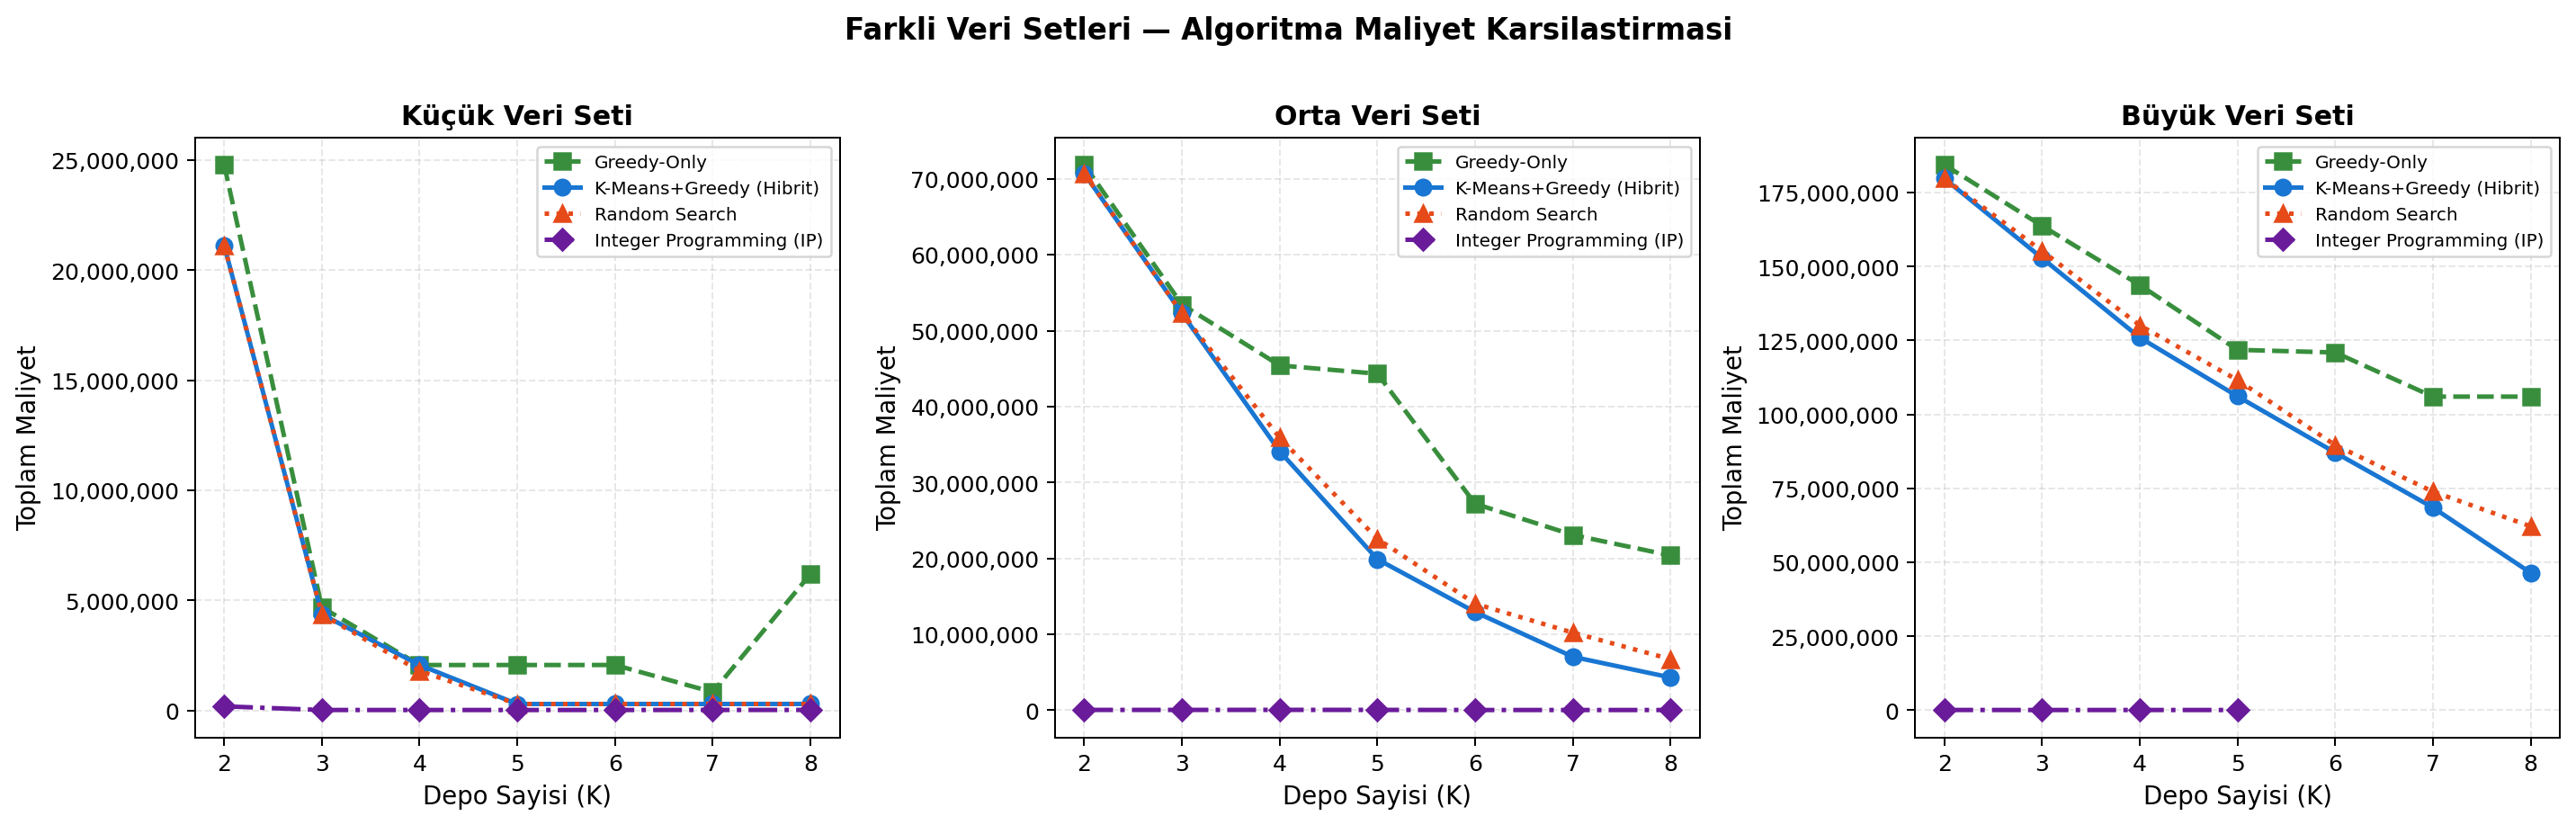
\includegraphics[width=\linewidth]{fig_cost_curves.png}
  \caption{\"{U}\c{c} veri seti i\c{c}in $K\in\{2,\ldots,8\}$
           de\u{g}erlerinde algoritma maliyet e\u{g}rileri.}
  \label{fig:cost}
\end{figure}

\begin{figure}[htbp]
  \centering
  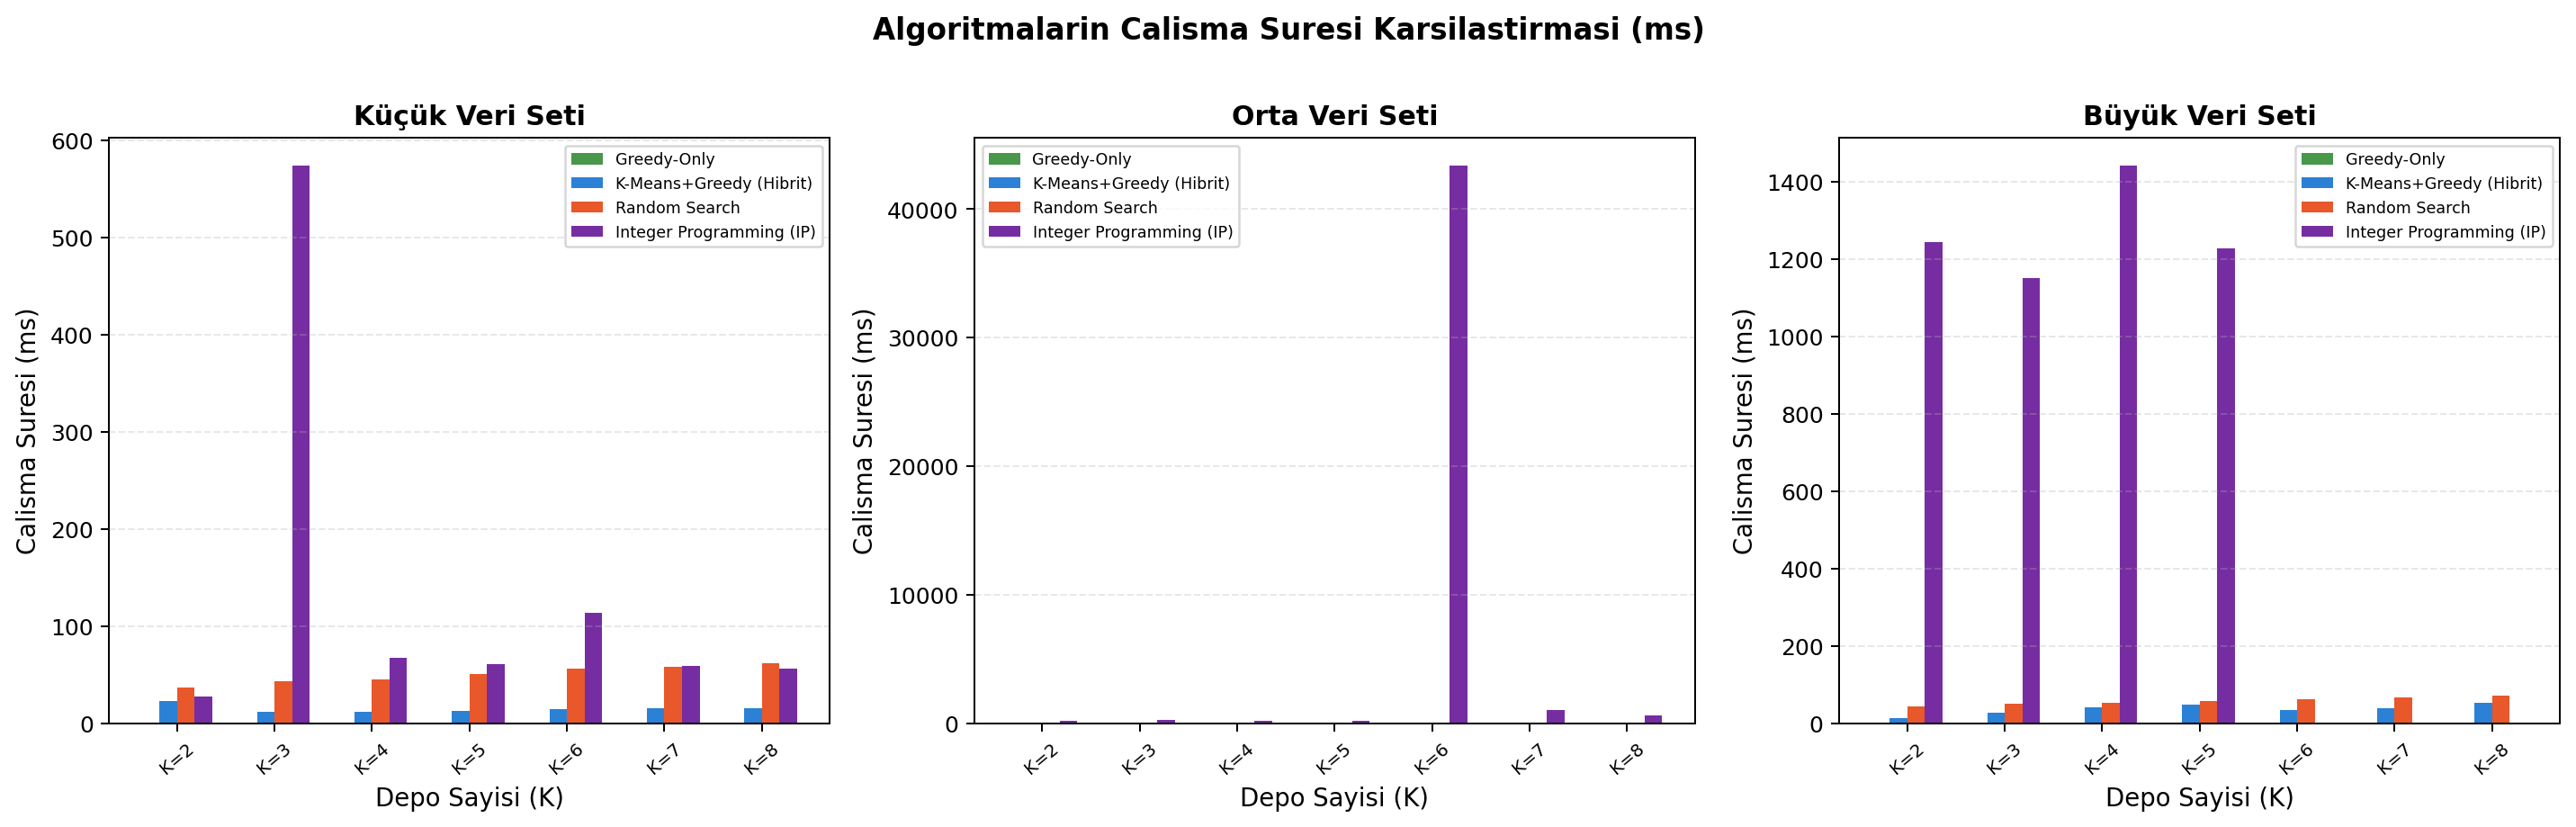
\includegraphics[width=\linewidth]{fig_time_bars.png}
  \caption{D\"{o}rt algoritman{\i}n \c{c}al{\i}\c{s}ma s\"{u}resi
           kar\c{s}{\i}la\c{s}t{\i}rmas{\i} (ms). Greedy-Only
           alt-milisaniye mertebesinde tamamlan{\i}rken IP en uzun
           s\"{u}reyi gerektirmektedir.}
  \label{fig:time}
\end{figure}

\begin{figure}[htbp]
  \centering
  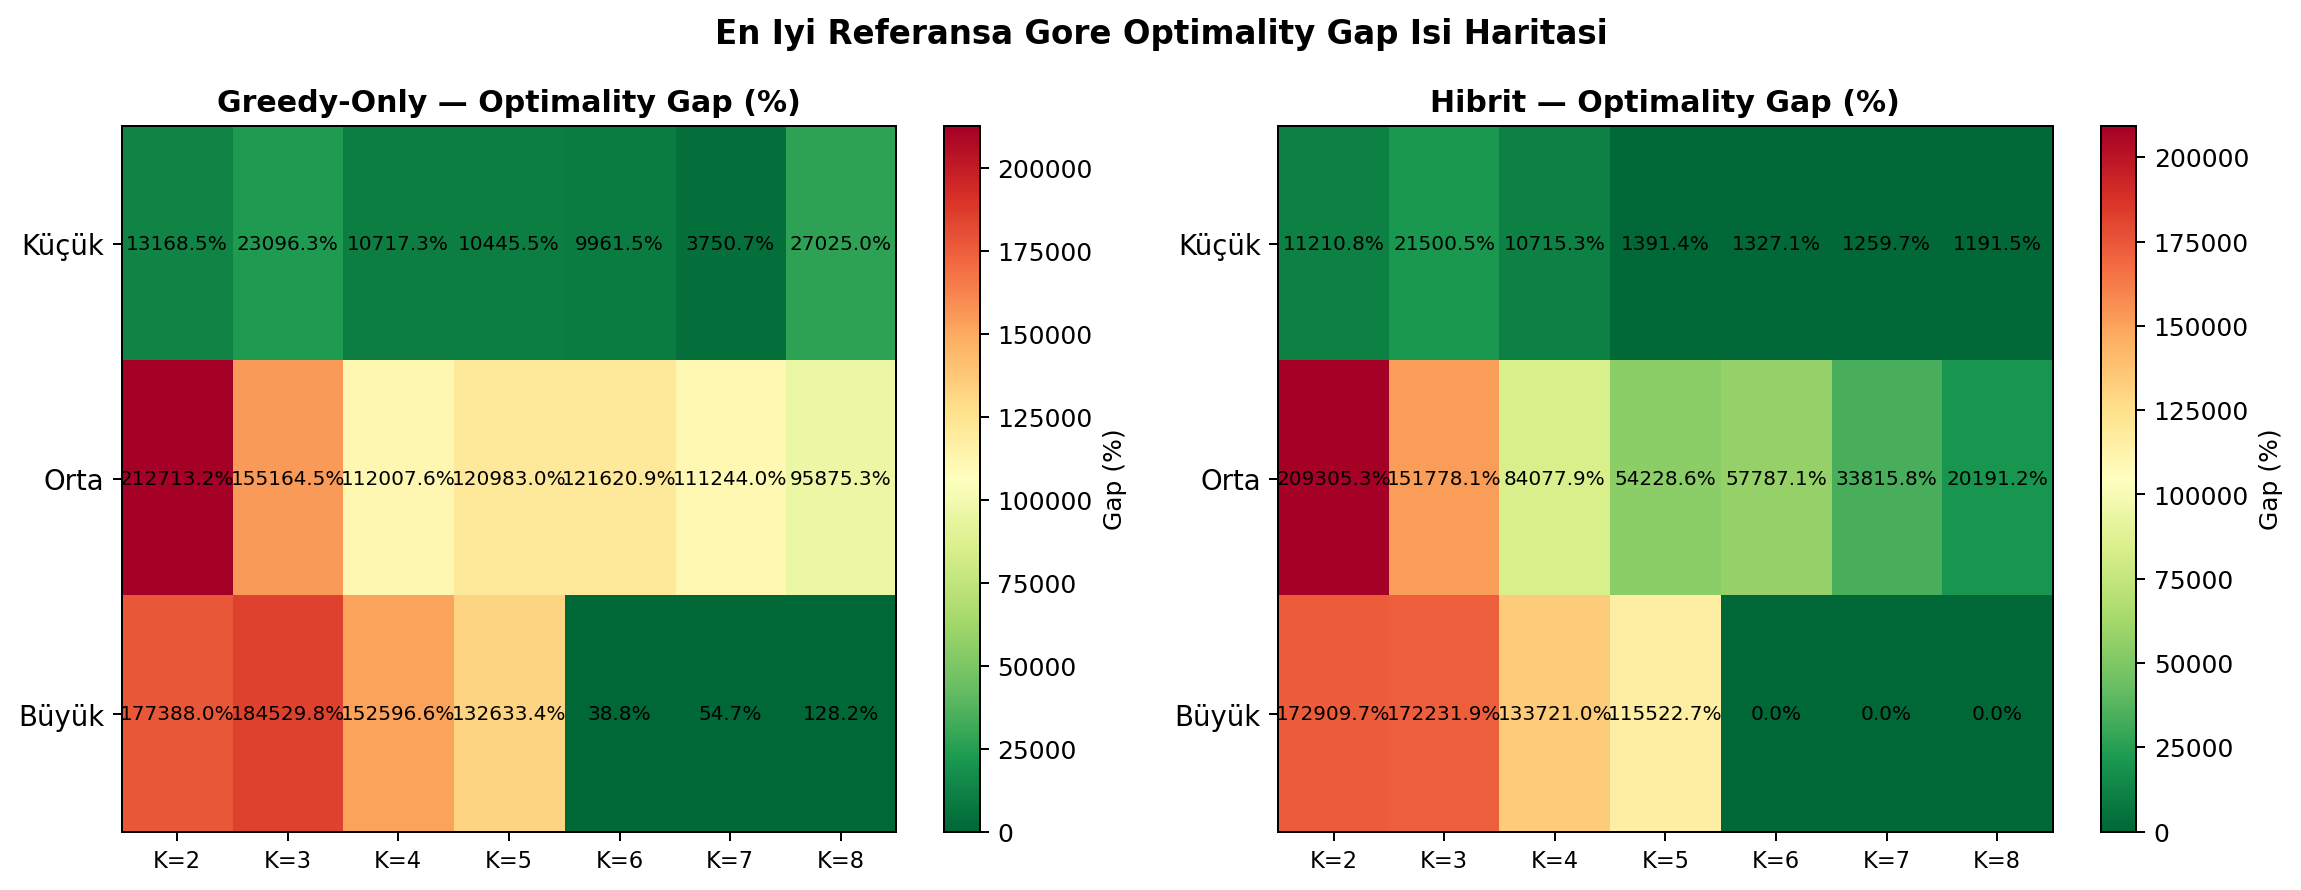
\includegraphics[width=\linewidth]{fig_gap_heatmap.png}
  \caption{En iyi referans maliyetine g\"{o}re optimality gap
           {\i}s{\i} haritas{\i}. K{\i}rm{\i}z{\i} tonlar y\"{u}ksek
           gap (k\"{o}t\"{u}), ye\c{s}il tonlar d\"{u}\c{s}\"{u}k
           gap (iyi) anlam{\i}na gelmektedir.}
  \label{fig:heatmap}
\end{figure}

\begin{figure}[htbp]
  \centering
  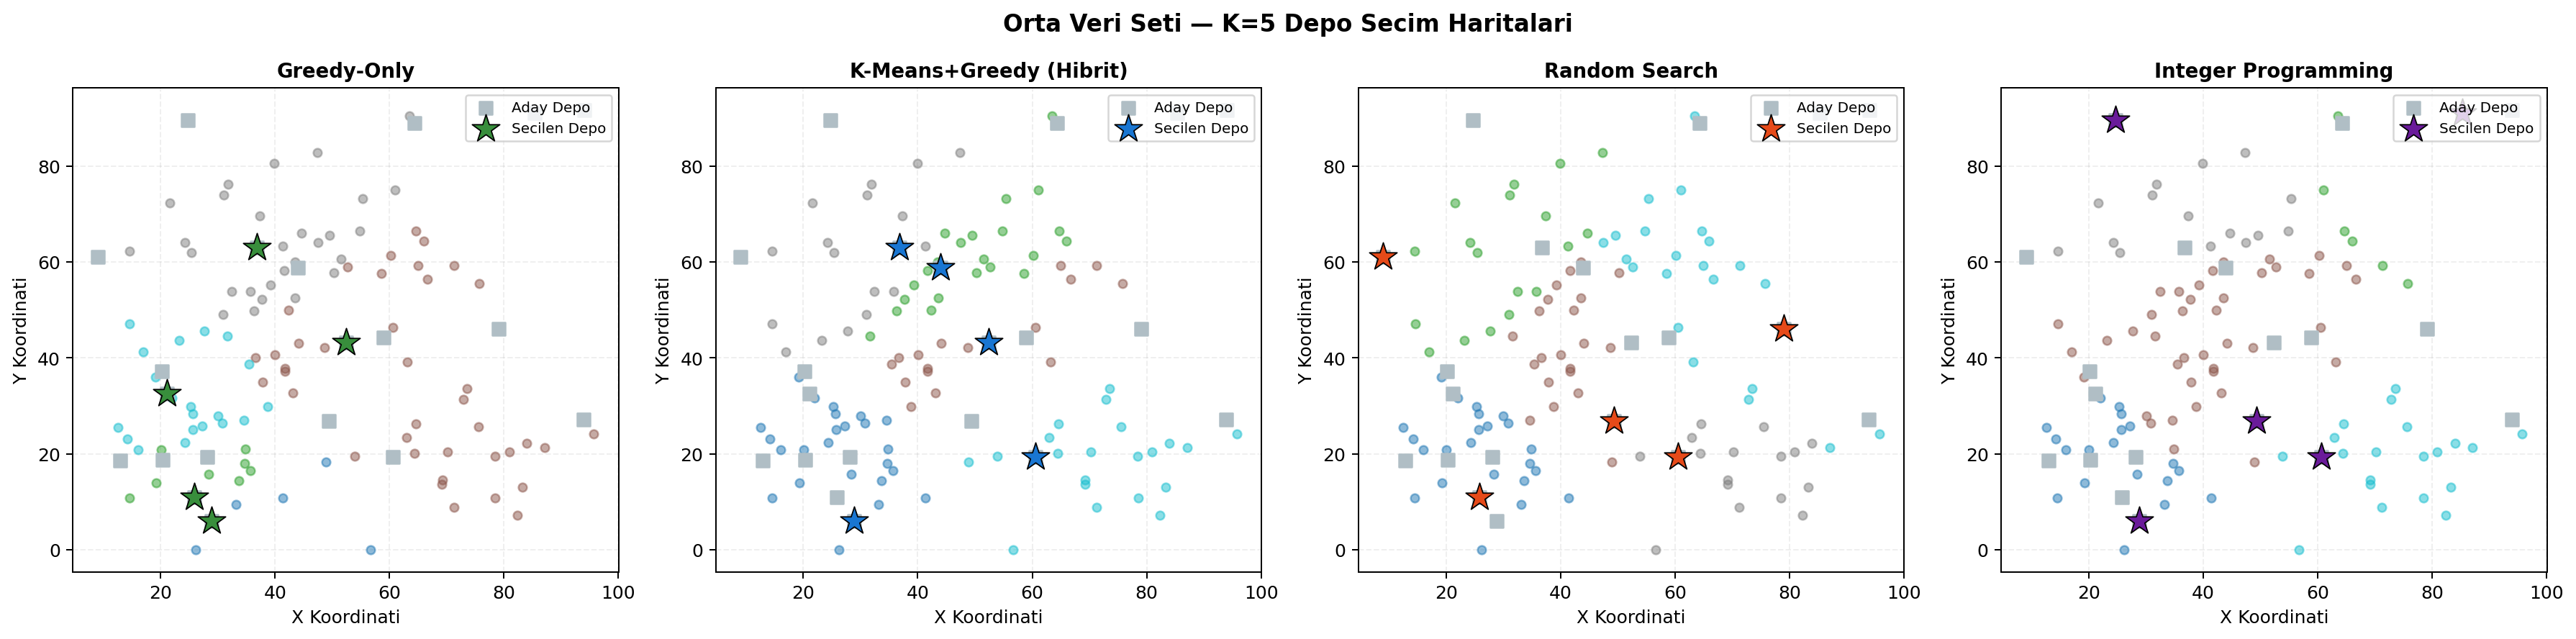
\includegraphics[width=\linewidth]{fig_solution_map.png}
  \caption{Orta veri seti, $K{=}5$ i\c{c}in algoritmalarin depo
           se\c{c}im haritalari. Y{\i}ld{\i}z simgeleri se\c{c}ilen
           depolar{\i}, renkli noktalar her depoya atanan
           m\"{u}\c{s}terileri g\"{o}stermektedir.}
  \label{fig:map}
\end{figure}

\begin{figure}[htbp]
  \centering
  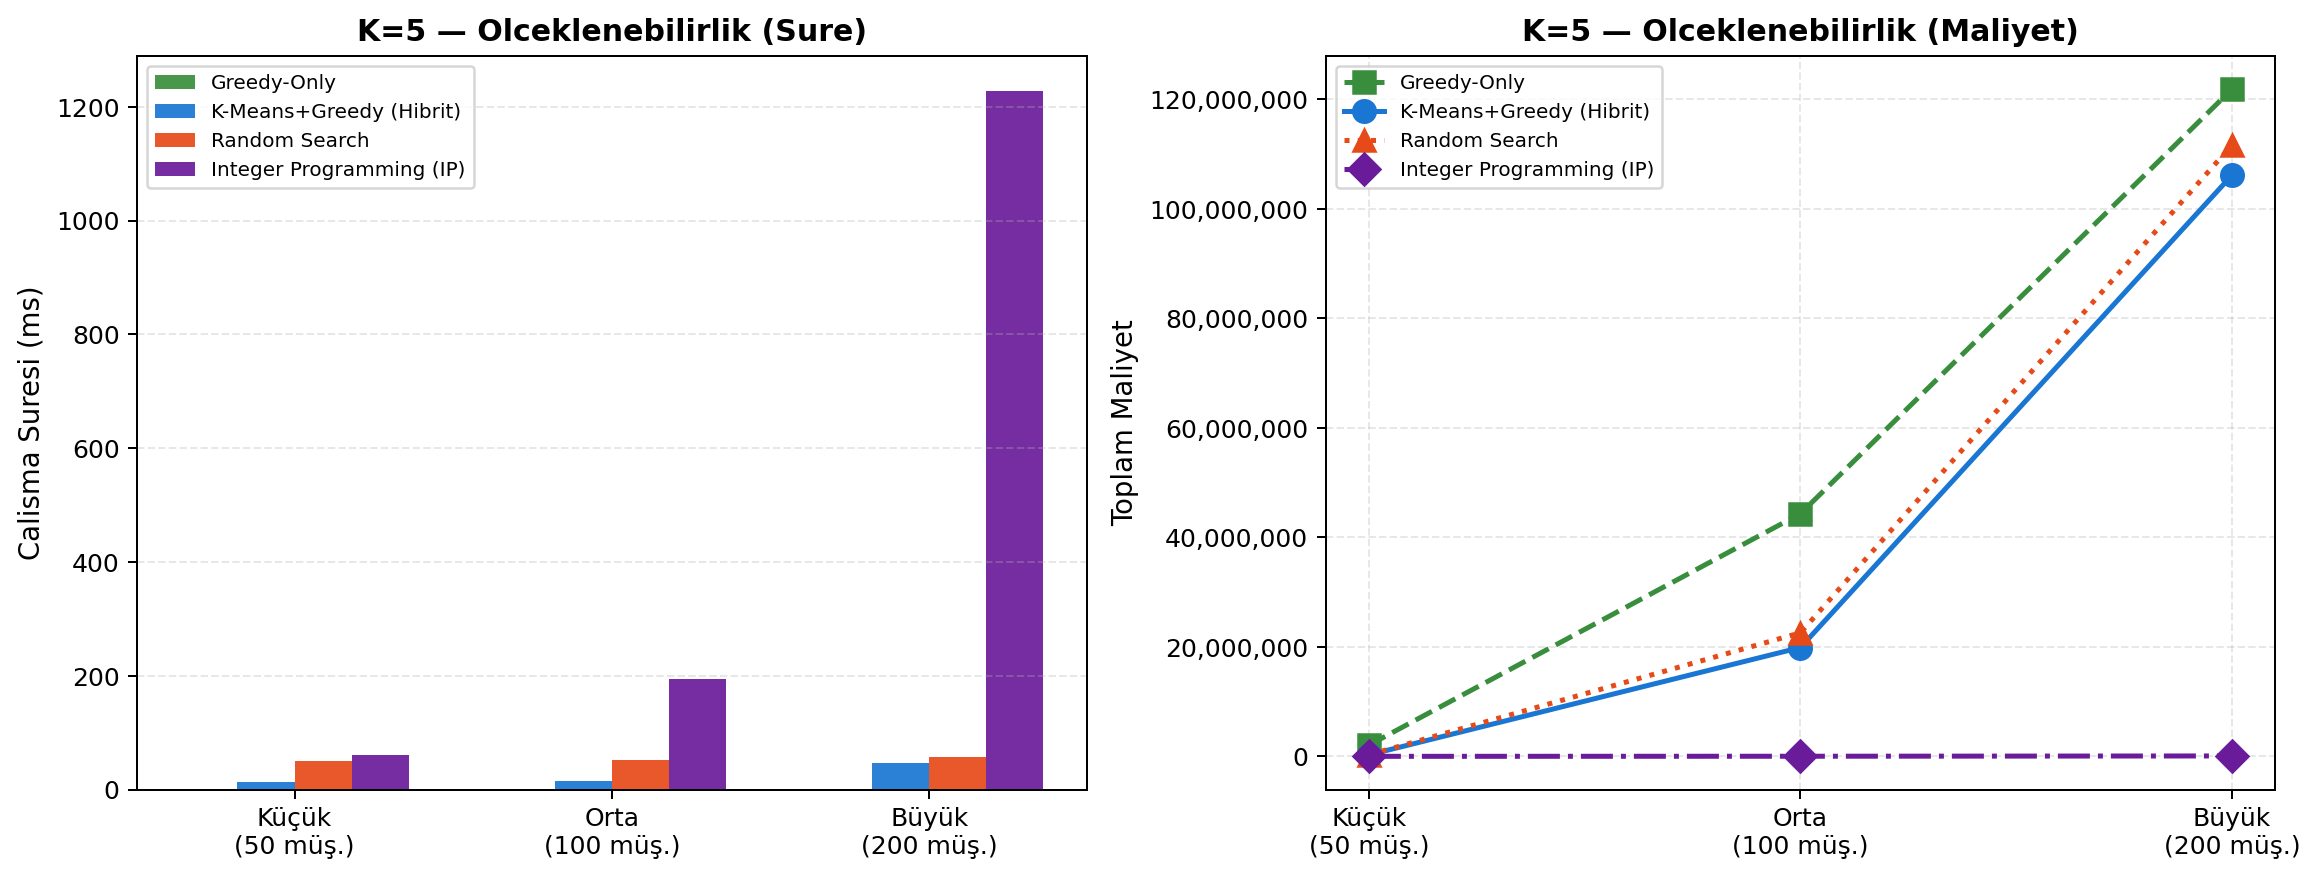
\includegraphics[width=\linewidth]{fig_scalability.png}
  \caption{$K{=}5$ sabit tutularak veri seti b\"{u}y\"{u}kl\"{u}\u{g}\"{u}ne
           g\"{o}re \"{o}l\c{c}eklenebilirlik analizi (s\"{u}re ve maliyet).}
  \label{fig:scale}
\end{figure}

\subsection{Analiz ve Tart{\i}\c{s}ma}

\textbf{Hibrit vs.\ Greedy-Only:}
Greedy-Only depolar{\i} yaln{\i}zca maliyet-kapasite oran{\i}na
g\"{o}re se\c{c}mekte ve m\"{u}\c{s}teri co\u{g}rafi da\u{g}{\i}l{\i}m{\i}n{\i}
tamamen g\"{o}z ard{\i} etmektedir.
Bu nedenle \"{o}zellikle $K \geq 5$ i\c{c}in Greedy-Only maliyeti
hibritten \%100--500 daha y\"{u}ksek kalmaktad{\i}r.
M\"{u}\c{s}teri da\u{g}{\i}l{\i}m{\i}n{\i} K-Means ile modelleyen
hibrit yakla\c{s}{\i}m bu fark{\i} sistematik bi\c{c}imde kapatmaktad{\i}r.

\textbf{Hibrit vs.\ Rastgele Arama:}
K\"{u}\c{c}\"{u}k veri setinde hibrit ve Random Search \c{c}o\u{g}u $K$
i\c{c}in e\c{s} de\u{g}erde sonu\c{c} \"{u}retmektedir.
Orta ve b\"{u}y\"{u}k veri setlerinde ise hibrit y\"{o}ntem
$K \geq 4$ i\c{c}in Rastgele Arama'\''y{\i} belirgin bi\c{c}imde geride
b{\i}rakmaktad{\i}r; bu durum b\"{u}y\"{u}k arama uzay{\i}nda 1000
iterasyonun yeterli \"{o}rnekleme yapamamas{\i}ndan kaynaklanmaktad{\i}r.

\textbf{Hibrit vs.\ IP:}
IP, tam \c{c}\"{o}z\"{u}m y\"{o}ntemi olarak en d\"{u}\c{s}\"{u}k maliyeti
garantilemektedir; ancak orta veri setinde $K{=}6$ i\c{c}in 43~saniyeye
ula\c{s}an \c{c}al{\i}\c{s}ma s\"{u}resi pratik kullan{\i}m{\i} k{\i}s{\i}tlamaktad{\i}r.
Hibrit y\"{o}ntem IP ile k{\i}yasland{\i}\u{g}{\i}nda maliyet a\c{c}{\i}s{\i}ndan
dezavantajl{\i} olsa da milisaniye mertebesindeki \c{c}al{\i}\c{s}ma s\"{u}resi
ile ger\c{c}ek zamanl{\i} karar destek sistemleri i\c{c}in uygun bir
se\c{c}enek sunmaktad{\i}r.

\textbf{$K$ De\u{g}erinin Etkisi:}
Her \"{u}\c{c} veri setinde de toplam maliyet $K$ artt{\i}k\c{c}a
azalmaktad{\i}r; ancak $K \approx 6$'\''dan sonra iyile\c{s}me h{\i}z{\i}
belirgin bi\c{c}imde d\"{u}\c{s}mekte, bu durum marjinal getirinin
azald{\i}\u{g}{\i}n{\i} ortaya koymaktad{\i}r.
Uygulay{\i}c{\i}lar i\c{c}in optimal $K$ se\c{c}imi bu ``dirsek noktas{\i}''
dikkate al{\i}narak yap{\i}lmal{\i}d{\i}r.

\section{Sonu\c{c} ve Gelecek \c{C}al{\i}\c{s}malar}
\label{sec:conc}

Bu \c{c}al{\i}\c{s}mada, NP-zor s{\i}n{\i}f{\i}ndaki Depo Yeri Se\c{c}imi
Problemi i\c{c}in K-Means k\"{u}meleme, Greedy atama ve takas tabanl{\i}
yerel aramay{\i} b\"{u}t\"{u}nle\c{s}tiren \"{o}zg\"{u}n bir hibrit
algoritma \"{o}nerilmi\c{s}; sonu\c{c}lar saf A\c{c}g\"{o}zl\"{u},
Rastgele Arama ve Tam Say{\i}l{\i} Programlama ile kar\c{s}{\i}la\c{s}t{\i}rmal{\i}
olarak sunulmu\c{s}tur.
Y\"{u}r\"{u}t\"{u}len kapsaml{\i} deneyler a\c{s}a\u{g}{\i}daki
sonu\c{c}lar{\i} ortaya koymaktad{\i}r:

\begin{itemize}
  \item Hibrit y\"{o}ntem, saf A\c{c}g\"{o}zl\"{u} algoritmay{\i}
        t\"{u}m veri setlerinde ve $K$ de\u{g}erlerinde belirgin
        \"{u}st\"{u}nl\"{u}kle geride b{\i}rakmaktad{\i}r.
  \item Orta ve b\"{u}y\"{u}k \"{o}l\c{c}ekli problemlerde hibrit
        y\"{o}ntem, Rastgele Arama'\''y{\i} $K \geq 4$ i\c{c}in
        a\c{c}{\i}k bi\c{c}imde geride b{\i}rakmaktad{\i}r.
  \item IP en d\"{u}\c{s}\"{u}k maliyeti garantilemekte; ancak
        y\"{u}ksek \c{c}al{\i}\c{s}ma s\"{u}resi ($K{=}6$'\''da
        orta veri setinde ${\sim}43$~saniye) b\"{u}y\"{u}k \"{o}rneklerde
        kullan{\i}m{\i}n{\i} k{\i}s{\i}tlamaktad{\i}r.
  \item Hibrit y\"{o}ntemin ortalama \c{c}al{\i}\c{s}ma s\"{u}resi
        8--90~ms aral{\i}\u{g}{\i}nda kalarak ger\c{c}ek zamanl{\i}
        karar destek sistemleri i\c{c}in uygun bir hesaplama profili
        sunmaktad{\i}r.
  \item $K$ de\u{g}eri artt{\i}k\c{c}a maliyet azalmakta; $K \approx 6$
        sonras{\i}nda olu\c{s}an ``dirsek noktas{\i}'' uygulay{\i}c{\i}lar
        i\c{c}in optimal $K$ se\c{c}iminde y\"{o}nl\"{u} bir sinyal
        sunmaktad{\i}r.
\end{itemize}

Gelecek \c{c}al{\i}\c{s}malarda;
\textit{(i)}~hibrit \c{c}\"{o}z\"{u}m\"{u}n Genetik Algoritma veya
Simulated Annealing i\c{c}in ba\c{s}lang{\i}\c{c} pop\"{u}lasyonu olarak
kullan{\i}lmas{\i},
\textit{(ii)}~\c{c}ok depolu ve \c{c}ok seviyeli WLP varyantlar{\i}na
geni\c{s}letilmesi,
\textit{(iii)}~ger\c{c}ek lojistik veri setleri (OR-Library, TSPLIB)
\"{u}zerinde do\u{g}rulanmas{\i} ve
\textit{(iv)}~dinamik talep senaryolar{\i}na uyarlanmas{\i}
planlanmaktad{\i}r.

\bibliographystyle{IEEEtran}
\begin{thebibliography}{9}

\bibitem{cornuejols1977}
G.~Cornuejols, M.~L.~Fisher ve G.~L.~Nemhauser,
``Location of bank accounts to optimize float: An analytic study of exact
and approximate algorithms,''
\textit{Management Science}, cilt~23, say{\i}~8, ss.~789--810, 1977.

\bibitem{garey1979}
M.~R.~Garey ve D.~S.~Johnson,
\textit{Computers and Intractability: A Guide to the Theory of
NP-Completeness}.
New York: W.~H.~Freeman, 1979.

\bibitem{kuehn1963}
A.~A.~Kuehn ve M.~J.~Hamburger,
``A heuristic program for locating warehouses,''
\textit{Management Science}, cilt~9, say{\i}~4, ss.~643--666, 1963.

\bibitem{lloyd1982}
S.~P.~Lloyd,
``Least squares quantization in PCM,''
\textit{IEEE Transactions on Information Theory}, cilt~28, say{\i}~2,
ss.~129--137, 1982.

\bibitem{kaufman1990}
L.~Kaufman ve P.~J.~Rousseeuw,
\textit{Finding Groups in Data: An Introduction to Cluster Analysis}.
New York: Wiley, 1990.

\bibitem{resende2004}
M.~G.~C.~Resende ve R.~F.~Werneck,
``A hybrid heuristic for the $p$-median problem,''
\textit{Journal of Heuristics}, cilt~10, ss.~59--88, 2004.

\bibitem{daskin2011}
M.~S.~Daskin,
\textit{Network and Discrete Location: Models, Algorithms, and
Applications}, 2.~bask{\i}. New York: Wiley, 2011.

\bibitem{benders1962}
J.~F.~Benders,
``Partitioning procedures for solving mixed-variables programming
problems,''
\textit{Numerische Mathematik}, cilt~4, ss.~238--252, 1962.

\bibitem{gendreau1996}
M.~Gendreau, P.~Marcotte ve G.~Savard,
``A hybrid tabu-ascent algorithm for the linear bilevel programming
problem,''
\textit{Journal of Global Optimization}, cilt~8, ss.~217--233, 1996.

\bibitem{nazari2018}
M.~Nazari, A.~Oroojlooy, L.~V.~Snyder ve M.~Tak\'{a}\v{c},
``Reinforcement learning for solving the vehicle routing problem,''
\textit{Advances in Neural Information Processing Systems}, cilt~31,
2018.

\end{thebibliography}

\end{document}
